%\renewcommand{\theequation}{\theenumi}
%\begin{enumerate}[label=\arabic*.,ref=\theenumi]
\begin{enumerate}[label=\thesection.\arabic*.,ref=\thesection.\theenumi]
\numberwithin{equation}{enumi}
\solution
From 
		\eqref{eq:geo-dir-vec-ab},
		\eqref{eq:geo-dir-vec-bc},
		\eqref{eq:geo-dir-vec-ca},
	\eqref{eq:median-d},
	\eqref{eq:median-e}
	and
	\eqref{eq:median-f},
\begin{align}
\vec{\frac{\vec{B}+\vec{C}}{2}} &= \frac{1}{2}\myvec{-{7} \\ 1},\,
\vec{B}-\vec{C} = \myvec{-1 \\ 11} 
\\
\vec{\frac{\vec{A}+\vec{B}}{2}}&=\frac{1}{2}\myvec{-{3} \\{5}},\,
\vec{A}-\vec{B}=\myvec{5\\ -7} \\
\vec{\frac{\vec{C}+\vec{A}}{2}} &= \myvec{-1\\-3},\,
\vec{C}-\vec{A} = \myvec{-4\\-4} \\
\end{align}
yielding
\begin{alignat}{2}
  \brak{\vec{B}-\vec{C}}^{\top}\brak{\frac{\vec{B}+\vec{C}}{2}}
	&=\myvec{-1&11}\myvec{-\frac{7}{2} \\ \frac{1}{2}}
	&&=9
  \\
\brak{\vec{A}-\vec{B}}^{\top}\brak{\frac{\vec{A}+\vec{B}}{2}}
	&=\myvec{5&-7}\myvec{-\frac{3}{2} \\\frac{5}{2}}
	&&=-25
  \\
\brak{\vec{C}-\vec{A}}^{\top}\brak{\frac{\vec{C}+\vec{A}}{2}}
	&=\myvec{-4&-4}\myvec{-1\\-3}
	&&=16
\end{alignat}
Thus, the perpendicular bisectors are obtained from 
			\eqref{eq:tri-perp-bisect}
			as
		\begin{alignat}{2}
			BC&: \quad \myvec{-1&11}\vec{x}&&=9
\\
			CA&: \quad \myvec{5&-7}\vec{x}&&=-25
\\
			AB&: \quad \myvec{-4&-4}\vec{x}&&=16
		\end{alignat}
\begin{figure}
\centering
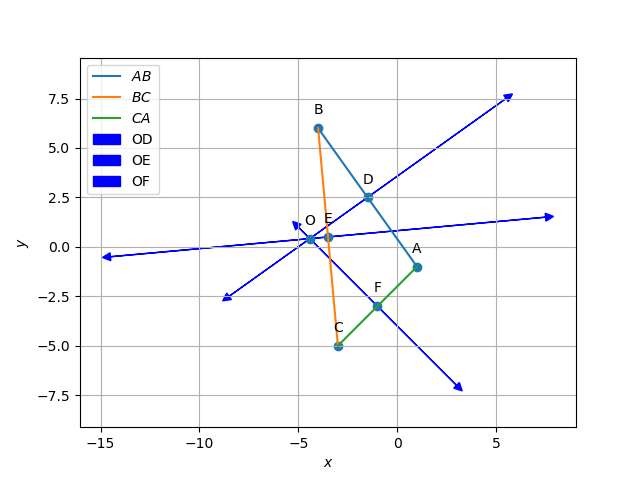
\includegraphics[width=\columnwidth]{solutions/1/4/1/figs/trianglecircum.png}
\caption{Plot of the perpendicular bisectors}
\label{fig:figure1}
\end{figure}




\item The equation of the perpendicular bisector of $BC$ is
		\begin{align}
			\label{eq:tri-perp-bisect}
			\brak{\vec{x}-\frac{\vec{B}+\vec{C}}{2}}\brak{\vec{B}-\vec{C}} = 0
		\end{align}
		Substitute numerical values and find the equations of the perpendicular bisectors of $AB, BC$ and $CA$.
	\item Find the intersection $\vec{O}$ of the perpendicular bisectors of $AB$ and $AC$.
 \\
 \solution \\
The intersection of 
			\eqref{eq:tri-perp-bisect-ca}
			and
			\eqref{eq:tri-perp-bisect-ab},
			can be obtained as
\begin{align}
\myvec{5&-7&-25\\1&1&-4} \xleftrightarrow[]{R_2 \leftarrow 5R_2 - R_1} \myvec{5&-7&-25\\0&12&5}\\
 \xleftrightarrow[]{R_1\leftarrow \frac{12}{7}R_1 + R_2} \myvec{\frac{60}{7}&0& \frac{-265}{7}\\0&12&5}
 \xleftrightarrow[R_1\leftarrow \frac{7}{60}R_1]{R_2 \leftarrow \frac{1}{12}R_2} \myvec{1&0& \frac{-53}{12}\\0&1&\frac{5}{12}}\\
\implies \vec{O}=\myvec{\frac{-53}{12}\\\frac{5}{12}}
			\label{eq:tri-perp-bisect-O}
\end{align}

	\item Verify that $\vec{O}$ satisfies
			\eqref{eq:tri-perp-bisect}.
$\vec{O}$ is known as the circumcentre.\\
    \solution
Substituing  from 
			\eqref{eq:tri-perp-bisect-O} in 
			\eqref{eq:tri-perp-bisect},
when substituted in the above equation,
\begin{multline}
	\brak{\vec{O}-\frac{\vec{B}+\vec{C}}{2}}^{\top}\brak{\vec{B}-\vec{C}}\\
	=\brak{\frac{1}{12}\myvec{-53\\5}- \frac{1}{2}\myvec{-7\\1}}^{\top} \myvec{-1\\11}\\
	=\frac{1}{12}\myvec{-11&-1}\myvec{-1\\11}
	=0
\end{multline}




		\item Verify that 
		\begin{align}
			OA = OB = OC 
		\end{align}
	\item Draw the circle with centre at $\vec{O}$ and radius 
		\begin{align}
			R = OA
		\end{align}
		This is known as the {\em circumradius}. 
  \\  \solution 
See 
\figref{fig:circumcircle with centre O}.
\begin{figure}
\centering
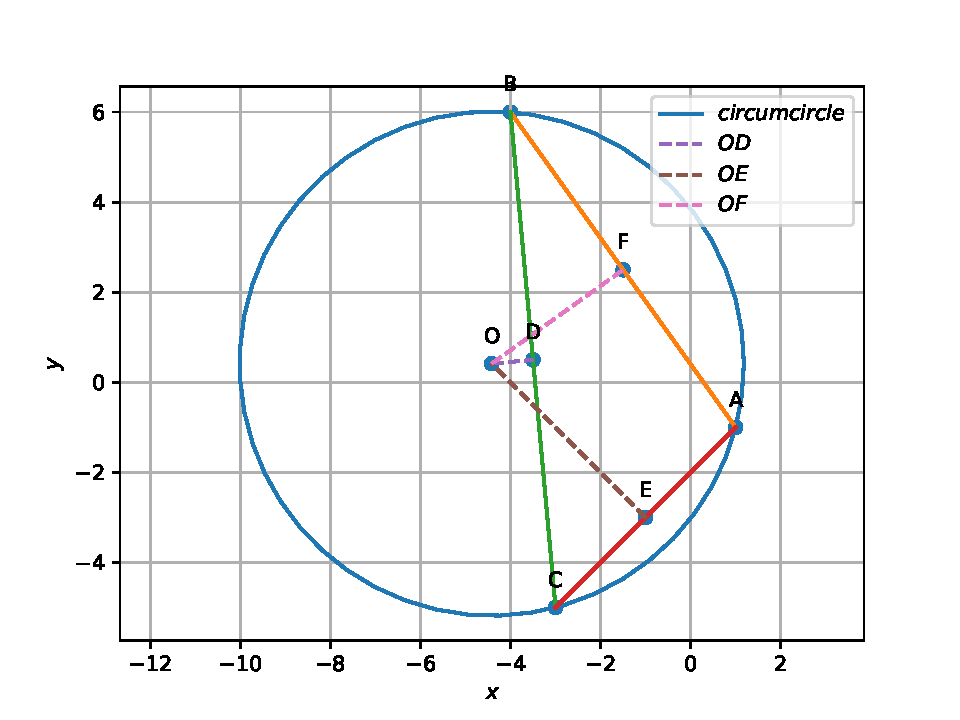
\includegraphics[width=\columnwidth]{figs/triangle/perp-bisect.pdf}
	\caption{Circumcircle of $\triangle ABC$ with centre $\vec{O}$.}
\label{fig:circumcircle with centre O}	
\end{figure}


	\item Verify that 
		\begin{align}
			\angle BOC = 2\angle BAC.
		\end{align}\\
  \solution
\begin{enumerate}
\item To find  the value of $\angle{BOC}$ :
\begin{align}
\vec{B}-\vec{O}
          &=\myvec{\frac{5}{12}\\\frac{67}{12}},\,
\vec{C}-\vec{O}
          =\myvec{\frac{17}{12}\\\frac{-65}{12}}
	  \\
\implies \brak{\vec{B}-\vec{O}}^{\top}\brak{\vec{C}-\vec{O}}&=\frac{-4270}{144}\\
	\implies \norm{\vec{B}-\vec{O}}&= \frac{\sqrt{4514}}{12},\,
	\norm{\vec{C}-\vec{O}}= \frac{\sqrt{4514}}{12}
\end{align}
Thus,
\begin{align}
\cos{BOC}&=\frac{\brak{\vec{B}-\vec{O}}^{\top}\brak{\vec{C}-\vec{O}}}{\norm{\vec{B}-\vec{O}}\norm{\vec{C}-\vec{O}}}
=\frac{-4270}{4514}\\
\implies\angle{BOC}&=\cos^{-1}\brak{\frac{-4270}{4514}}
\\
	&=161.07536\degree
	\text{ or }
	198.92464\degree\label{eq:1}
\end{align}
	\item To find  the value of $\angle{BAC}$ :
\begin{align}
\vec{B}-\vec{A}&=\myvec{-5\\7},\,
\vec{C}-\vec{A}=\myvec{-4\\-4}
\\
\implies \brak{\vec{B}-\vec{A}}^{\top}\brak{\vec{C}-\vec{A}}&=-8
\\
	\norm{\vec{B}-\vec{A}}&= \sqrt{74}
	\norm{\vec{C}-\vec{A}}= 4\sqrt{2}
\end{align}
Thus,
\begin{align}
\cos{BAC}&=\frac{\brak{\vec{B}-\vec{A}}^{\top}\brak{\vec{C}-\vec{A}}}{\norm{\vec{B}-\vec{A}}\norm{\vec{C}-\vec{A}}}
=\frac{-8}{4\sqrt{148}}\\
\implies\angle{BAC}&=\cos^{-1}\brak{\frac{-8}{4\sqrt{148}}}\\
&=99.46232\degree \label{eq:2}
\end{align}
From \eqref{eq:2} and \eqref{eq:1},
\begin{align}
2\times\angle{BAC}
= \angle{BOC}
\end{align}
\end{enumerate}





	\item Let 
		\begin{align}
			\vec{P} = \myvec{\cos \theta & -\sin \theta \\ \sin \theta & \cos \theta}
		\end{align}
		Find $\theta$ if 
		\begin{align}
			\vec{C}-\vec{O}=\vec{P}\brak{\vec{A}-\vec{O}}
		\end{align}
\end{enumerate}
